\documentclass[]{article}
\usepackage{lmodern}
\usepackage{amssymb,amsmath}
\usepackage{ifxetex,ifluatex}
\usepackage{fixltx2e} % provides \textsubscript
\ifnum 0\ifxetex 1\fi\ifluatex 1\fi=0 % if pdftex
  \usepackage[T1]{fontenc}
  \usepackage[utf8]{inputenc}
\else % if luatex or xelatex
  \ifxetex
    \usepackage{mathspec}
  \else
    \usepackage{fontspec}
  \fi
  \defaultfontfeatures{Ligatures=TeX,Scale=MatchLowercase}
\fi
% use upquote if available, for straight quotes in verbatim environments
\IfFileExists{upquote.sty}{\usepackage{upquote}}{}
% use microtype if available
\IfFileExists{microtype.sty}{%
\usepackage{microtype}
\UseMicrotypeSet[protrusion]{basicmath} % disable protrusion for tt fonts
}{}
\usepackage[margin=1in]{geometry}
\usepackage{hyperref}
\hypersetup{unicode=true,
            pdftitle={Trabajo Curso Series de Tiempo},
            pdfauthor={Eduardo Contreras Bohórquez},
            pdfborder={0 0 0},
            breaklinks=true}
\urlstyle{same}  % don't use monospace font for urls
\usepackage{longtable,booktabs}
\usepackage{graphicx,grffile}
\makeatletter
\def\maxwidth{\ifdim\Gin@nat@width>\linewidth\linewidth\else\Gin@nat@width\fi}
\def\maxheight{\ifdim\Gin@nat@height>\textheight\textheight\else\Gin@nat@height\fi}
\makeatother
% Scale images if necessary, so that they will not overflow the page
% margins by default, and it is still possible to overwrite the defaults
% using explicit options in \includegraphics[width, height, ...]{}
\setkeys{Gin}{width=\maxwidth,height=\maxheight,keepaspectratio}
\IfFileExists{parskip.sty}{%
\usepackage{parskip}
}{% else
\setlength{\parindent}{0pt}
\setlength{\parskip}{6pt plus 2pt minus 1pt}
}
\setlength{\emergencystretch}{3em}  % prevent overfull lines
\providecommand{\tightlist}{%
  \setlength{\itemsep}{0pt}\setlength{\parskip}{0pt}}
\setcounter{secnumdepth}{0}
% Redefines (sub)paragraphs to behave more like sections
\ifx\paragraph\undefined\else
\let\oldparagraph\paragraph
\renewcommand{\paragraph}[1]{\oldparagraph{#1}\mbox{}}
\fi
\ifx\subparagraph\undefined\else
\let\oldsubparagraph\subparagraph
\renewcommand{\subparagraph}[1]{\oldsubparagraph{#1}\mbox{}}
\fi

%%% Use protect on footnotes to avoid problems with footnotes in titles
\let\rmarkdownfootnote\footnote%
\def\footnote{\protect\rmarkdownfootnote}

%%% Change title format to be more compact
\usepackage{titling}

% Create subtitle command for use in maketitle
\newcommand{\subtitle}[1]{
  \posttitle{
    \begin{center}\large#1\end{center}
    }
}

\setlength{\droptitle}{-2em}

  \title{Trabajo Curso Series de Tiempo}
    \pretitle{\vspace{\droptitle}\centering\huge}
  \posttitle{\par}
    \author{Eduardo Contreras Bohórquez}
    \preauthor{\centering\large\emph}
  \postauthor{\par}
    \date{}
    \predate{}\postdate{}
  

\begin{document}
\maketitle

{
\setcounter{tocdepth}{2}
\tableofcontents
}
\section{Estadísticas descriptivas}\label{estadisticas-descriptivas}

Serie de tiempo del número de heridos en la base de datos de accidentes.
163 registros mensuales desde enero de 2005 hasta julio de 2018.

\includegraphics{Trabajo_files/figure-latex/unnamed-chunk-2-1.pdf}

\section{Transformación Box-Cox para estabilizar la
varianza}\label{transformacion-box-cox-para-estabilizar-la-varianza}

Aunque en la serie original no se observa un problema de
heterocedasticidad severo, se aplicó la transformación BoxCox con el
parámetro lambda = 2 obtenido a través del método BoxCox.lambda de R.

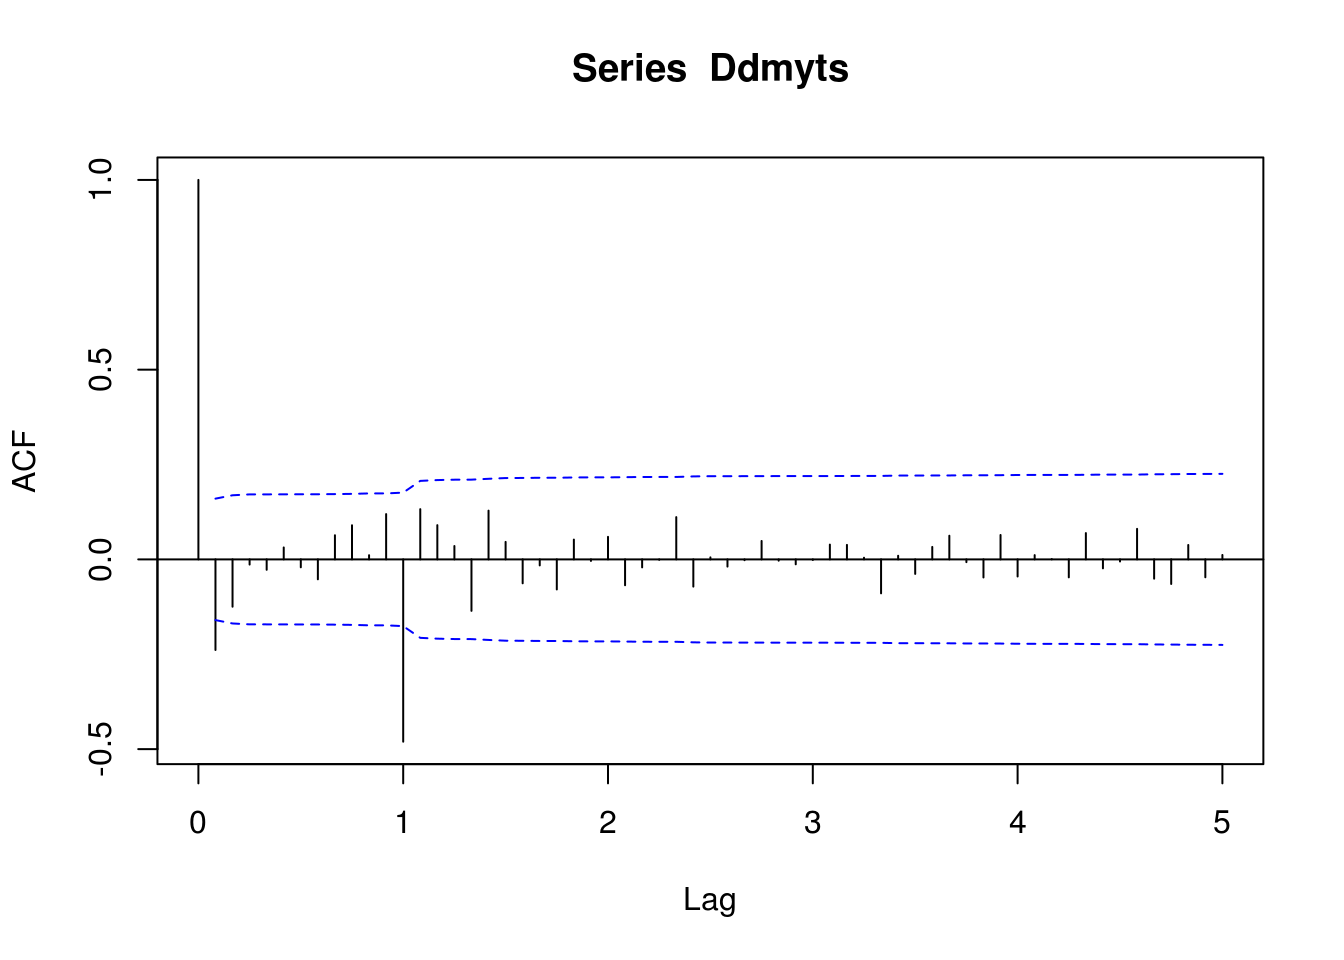
\includegraphics{Trabajo_files/figure-latex/unnamed-chunk-3-1.pdf}

\section{Descomposición de la serie}\label{descomposicion-de-la-serie}

El diagrama de autocorrelación muestra que se presenta una asociación
estadística entre el numero de heridos en el tiempo t, y los heridos a
un rezago de tiempo h, esto se presenta inclusive a rezagos de más de 5
años como se observa en la gráfica.

\includegraphics{Trabajo_files/figure-latex/unnamed-chunk-4-1.pdf}

Se aplica diferenciación para remover la tendencia y estacionaliad de la
serie.

\includegraphics{Trabajo_files/figure-latex/unnamed-chunk-5-1.pdf}

\includegraphics{Trabajo_files/figure-latex/unnamed-chunk-6-1.pdf}

\section{Pruebas de raíces unitarias}\label{pruebas-de-raices-unitarias}

El test de Dickey-Fuller de raíces unitarias sobre la serie que ha
pasado por los procesos de estabilización de la varianza y
diferenciación para remover tendencia y estacionalidad, indica que la
componente restante es estacionaria con un nivel de confianza del 95\%.

\includegraphics{Trabajo_files/figure-latex/unnamed-chunk-8-1.pdf}

\section{Postulación de modelos
ARIMA}\label{postulacion-de-modelos-arima}

\begin{itemize}
\tightlist
\item
  A partir del diagrama de autocorrelación simple se postula el modelo
  de Promedios móviles puro MA(1).
\item
  Mediante diagrama de autocorrelación parcial se postula el modelo
  Autorregresivo puro AR(2).
\item
  Con la función auto.arima de R, restringiendo los órdenes ordinarios
  max.p=2, max.q=1, y estacionales max.P=2 y max.Q=1 (de acuerdo a los
  correlogramas), se obtuvo el modelo ARIMA(1,0,0)(2,0,0){[}12{]} con
  media distinta de 0.
\end{itemize}

\includegraphics{Trabajo_files/figure-latex/unnamed-chunk-9-1.pdf}
\includegraphics{Trabajo_files/figure-latex/unnamed-chunk-9-2.pdf}

\section{Ajuste de modelos ARIMA}\label{ajuste-de-modelos-arima}

Mostrar tabla

\begin{longtable}[]{@{}lllllllll@{}}
\toprule
MODELO & BIC & RECM & Normalidad & No.auto.correlación &
Parametros.estables & Varianza.constante & Media.0 &\tabularnewline
\midrule
\endhead
ARIMA(0,1,1)(0,1,0){[}12{]} & & & & & & & &\tabularnewline
Box Cox transformation: lambda= 2 4601.49 429.0486 no & n & o & & no & &
& &\tabularnewline
Regression with ARIMA(0,1,1)(0,1,0){[}12{]} errors (outliers) & & & & &
& & &\tabularnewline
Box Cox transformation: lambda= 2 4539.24 no no & & & & & & &
&\tabularnewline
ARIMA(2,1,0)(0,1,0){[}12{]} & & & & & & & &\tabularnewline
Box Cox transformation: lambda= 2 4607.78 424.9401 no & n & o & & no & &
& &\tabularnewline
Regression with ARIMA(2,1,0)(0,1,0){[}12{]} errors (outliers) & & & & &
& & &\tabularnewline
Box Cox transformation: lambda= 2 4543.62 no & & & & & & &
&\tabularnewline
ARIMA(1,0,0)(2,0,0){[}12{]} with non-zero mean & & & & & & &
&\tabularnewline
Box Cox transformation: lambda= 2 4963.8 367.3052 no & & & & & & &
&\tabularnewline
Regression with ARIMA(1,0,0)(2,0,0){[}12{]} errors (outliers) & & & & &
& & &\tabularnewline
Box Cox transformation: lambda= 2 4936.63 & & & & & & & &\tabularnewline
ARIMA(1,1,0)(2,1,0){[}12{]} & & & & & & & &\tabularnewline
Box Cox transformation: lambda= 2 4565.51 345.3897 no & n & o & & & & &
&\tabularnewline
Regression with ARIMA(1,1,0)(2,1,0){[}12{]} errors & & & & & & &
&\tabularnewline
Box Cox transformation: lambda= 2 4528.52 no & & & no & & & &
&\tabularnewline
ARIMA(1,1,0)(2,1,0){[}12{]} & & & & & & & &\tabularnewline
Box Cox transformation: lambda= 3.172689 7410.35 326.2036 no & n & o & &
& & & &\tabularnewline
\bottomrule
\end{longtable}

Mostrar todo para el seleccionado - pronosticos - supuestos - rolling

Mostrar rolling para menor ECM


\end{document}
